\documentclass{article}
\usepackage[LGR, T1]{fontenc}
\usepackage[utf8]{inputenc}
\usepackage[greek,english]{babel}
\usepackage{alphabeta}
\usepackage{hyperref}
\usepackage{tikz} % Draw
\usepackage{wrapfig} % Potision plots
\usepackage{pgfplots} % Plot
\pgfplotsset{compat = newest}
\usepackage{amsmath} % AMS Math Package
\usepackage{graphicx} % Allows for eps images

\usepackage{float}
\usepackage{subcaption}

\title{Δίκτυα Υπολογιστών Ι - Session 1}
\author{Στεφανίδης Ιωάννης}
\date{ΑΕΜ: 9587}

\graphicspath{{../graphs/session1/}}

\begin{document}

\maketitle

\begin{figure}[H]
  \centering
  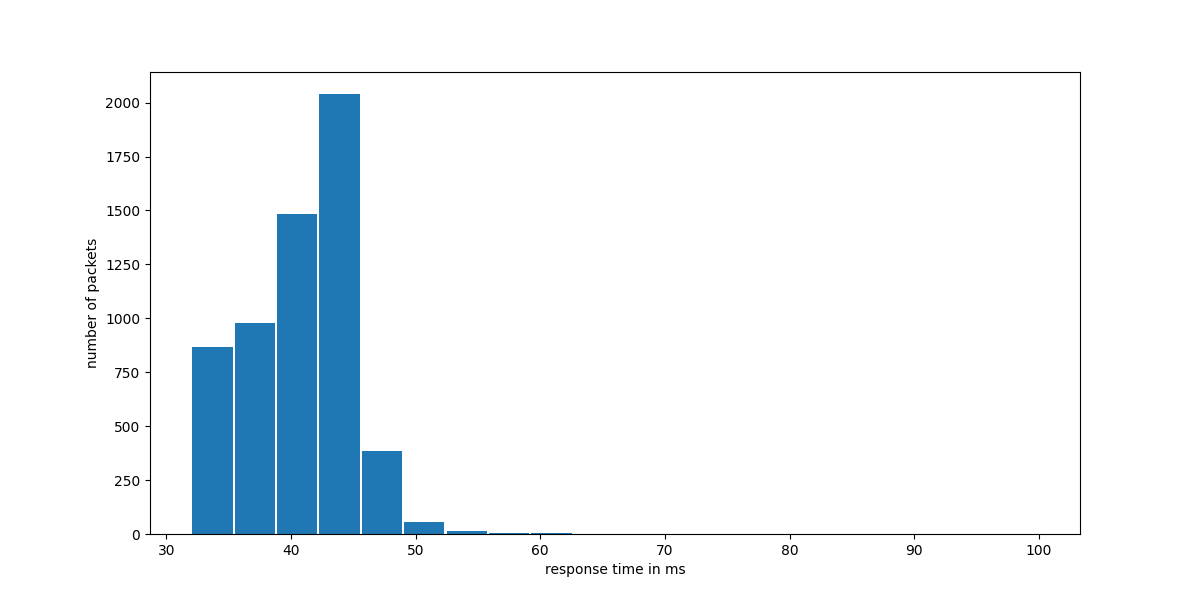
\includegraphics[width=\textwidth]{G1.png}
  \caption{Ιστόγραμμα G1}
  \label{fig:G1}
\end{figure}

\begin{figure}[H]
\begin{subfigure}{.5\textwidth}
  \centering
  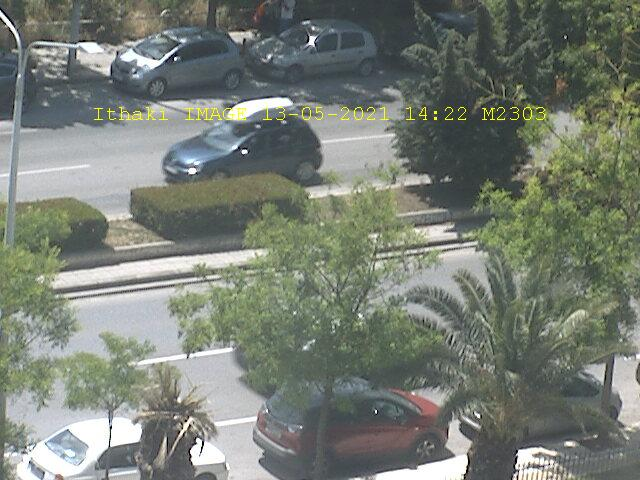
\includegraphics[width=0.9\linewidth]{image_M2303.jpg}
  \caption{E1}
  \label{fig:sfig1}
\end{subfigure}%
\begin{subfigure}{.5\textwidth}
  \centering
  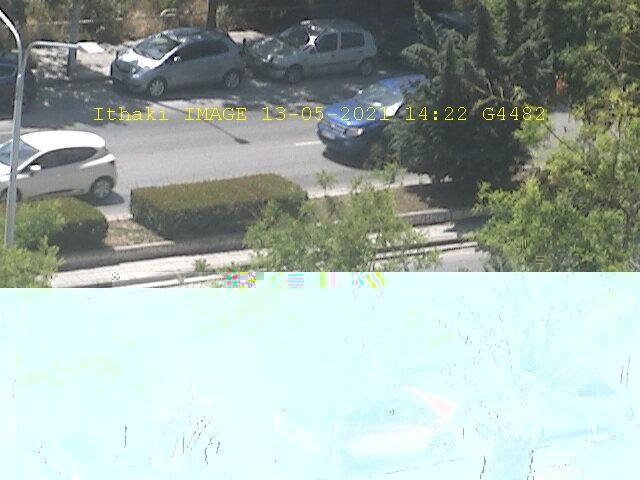
\includegraphics[width=0.9\linewidth]{image_G4482.jpg}
  \caption{E2}
  \label{fig:sfig2}
\end{subfigure}
\caption{Εικόνες απο κάμερα}
\label{fig:fig}
\end{figure}

\begin{figure}[H]
  \centering
  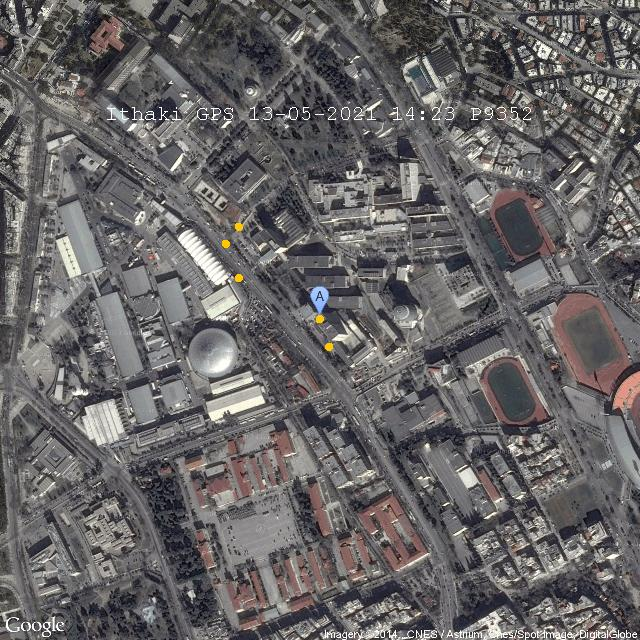
\includegraphics[width=\textwidth]{image_P9352T=225735403737T=225728403741T=225727403743T=225728403744.jpg}
  \caption{Εικόνα GPS Μ1}
  \label{fig:M1}
\end{figure}

\begin{figure}[H]
  \centering
  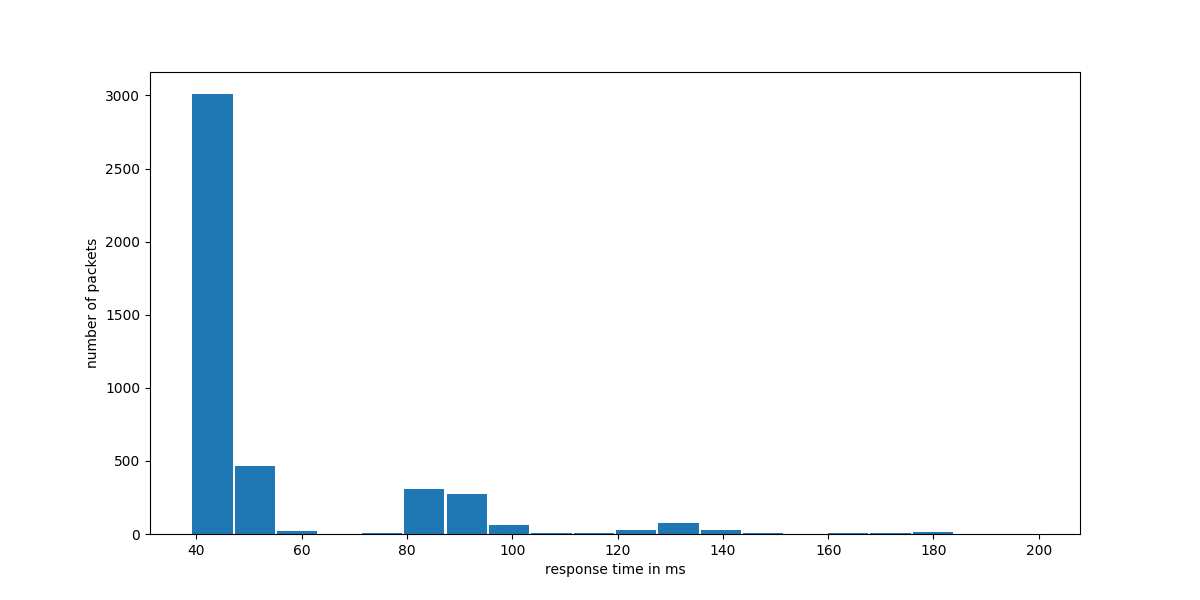
\includegraphics[width=\textwidth]{G2.png}
  \caption{Ιστόγραμμα G2}
  \label{fig:G2}
\end{figure}

\begin{figure}[H]
  \centering
  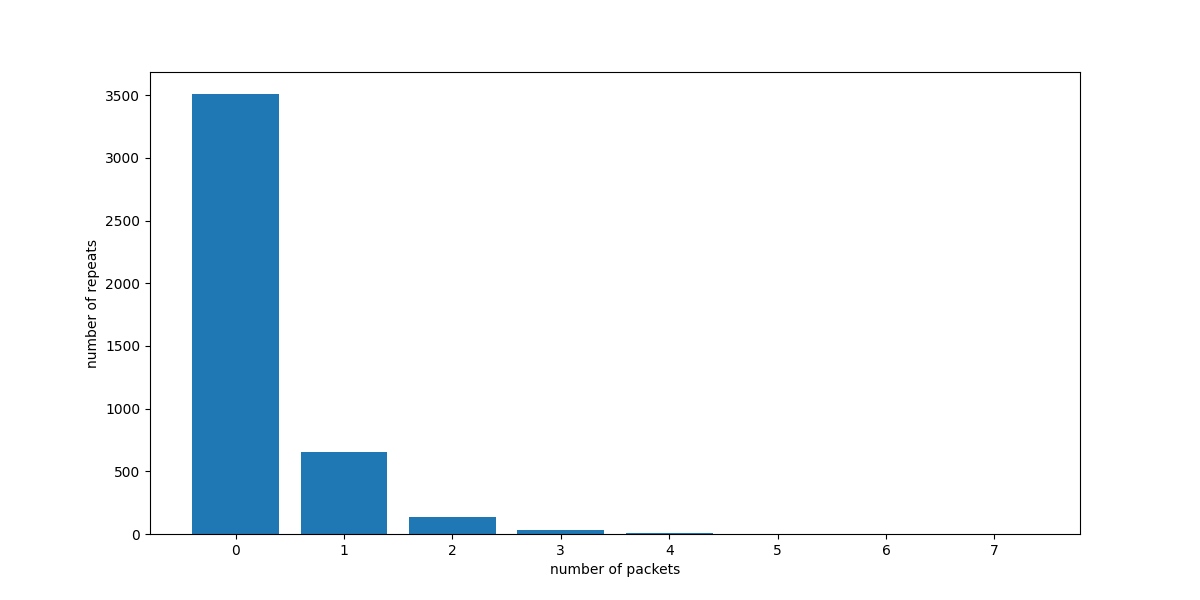
\includegraphics[width=\textwidth]{G3.png}
  \caption{Bar chart G3}
  \label{fig:G3}
\end{figure}


Όπως φαίνεται στο G3 η κατανομή πιθανότης του αριθμού επανεκπομπών είναι
γεωμετρική.
\\
Για το υπολογισμό του $BER$, βρίσκουμε τα ολικά bytes που πήραμε $B_T = 86240$
και τα πόσα από αυτά ήταν error bytes $B_E = 16832$. Άρα ορίζοντας $A =
\frac{B_T}{B_E} = 0.195$, υπολογίζουμε το $$BER = 1 - A^{1 /16} = 0.097$$

\pagebreak
\paragraph{Κωδικοί session}\hfill\\
ECHO -> E7901\\
IMAGE ERROR FREE -> M2303\\
IMAGE WITH ERROR -> G4482\\
GPS -> P9352\\
ACK -> Q7490\\
NACK -> R1469\\

\end{document}
